\documentclass{standalone}
\usepackage{tikz}
\begin{document}
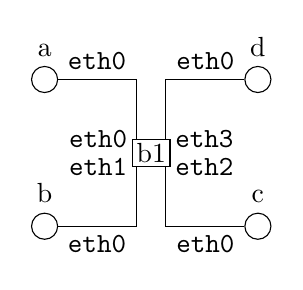
\begin{tikzpicture}
    \draw
    (0,0) node [rectangle, inner sep=1.5pt, draw](b1){b1}
    (b1.45)node[right]{\verb|eth3|}|-++(1,0.75)node[above left]{\verb|eth0|} node [draw, circle, anchor=west, label=d]{}
    (b1.315)node[right]{\verb|eth2|}|-++(1,-0.75)node[below left]{\verb|eth0|} node [draw, circle, anchor=west, label=c]{}
    (b1.225)node[left]{\verb|eth1|}|-++(-1,-0.75)node[below right]{\verb|eth0|} node [draw, circle, anchor=east,label=b]{}
    (b1.135)node[left]{\verb|eth0|}|-++(-1,0.75)node[above right]{\verb|eth0|} node [draw, circle, anchor=east,label=a]{}
    
    ;
\end{tikzpicture}
\end{document}